\documentclass[t,aspectratio=169]{beamer}
\usetheme{ffmodernneu}  %% Themenwahl

\usepackage[ngerman]{babel} 
\usepackage[T1]{fontenc}    % richtige Silbentrennung
\usepackage[utf8]{inputenc} % Umlaute etc.!
\usepackage{eurosym}
\usepackage{tikz}
\usepackage{pgffor}

\usetikzlibrary{arrows,decorations.pathmorphing,backgrounds,fit,positioning,shapes.symbols,chains}

%-----------------
\title{Über die Organisation und\\ Entwicklung von Freifunk}
\author{\newline\newline\newline\newline\newline\newline\newline\newline Matthias Marx und Leo Krüger}

\date{Forum Privatheit, 13. November 2020}
%\license{CC-BY-3.0}

\begin{document}
  \maketitle
  
  %-----------------  
  \begin{frame}{Was ist Freifunk?} 
    \begin{itemize}
      \item Initiative für freie, offene, kostenlose Netzwerke
      \item Nichtkommerzielles Netz in Nutzerhand
      \item Steht allen offen
      \item Nutzt freie, quelloffene Programme
      \item Netzneutral
    \end{itemize}
  \end{frame}
  
  %-----------------
  \begin{frame}{Verbreitung}
    \vspace{-2em}
    \begin{columns}
      \begin{column}{0.6\textwidth}
        \begin{itemize}
          \item Mehr als 50.000 Zugangspunkte an mehr als 400 Orten
          \item Zunehmend Unterstützung durch Bund und Länder
        \end{itemize}
      \end{column}
      \begin{column}{0.4\textwidth}
        \begin{center}
          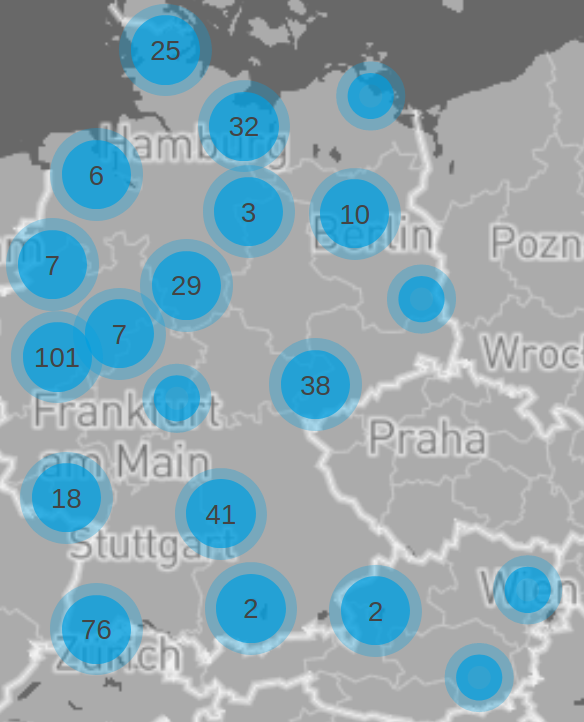
\includegraphics[height=0.8\textheight]{Bilder/community-map-2020-11-12}
        \end{center}
      \end{column}
    \end{columns}
  \end{frame}
  
  %----------------- 
  \begin{frame}{Freifunkknoten}
        \vspace{-2em}
    \begin{columns}
      \begin{column}{0.4\textwidth}
        \begin{center}
          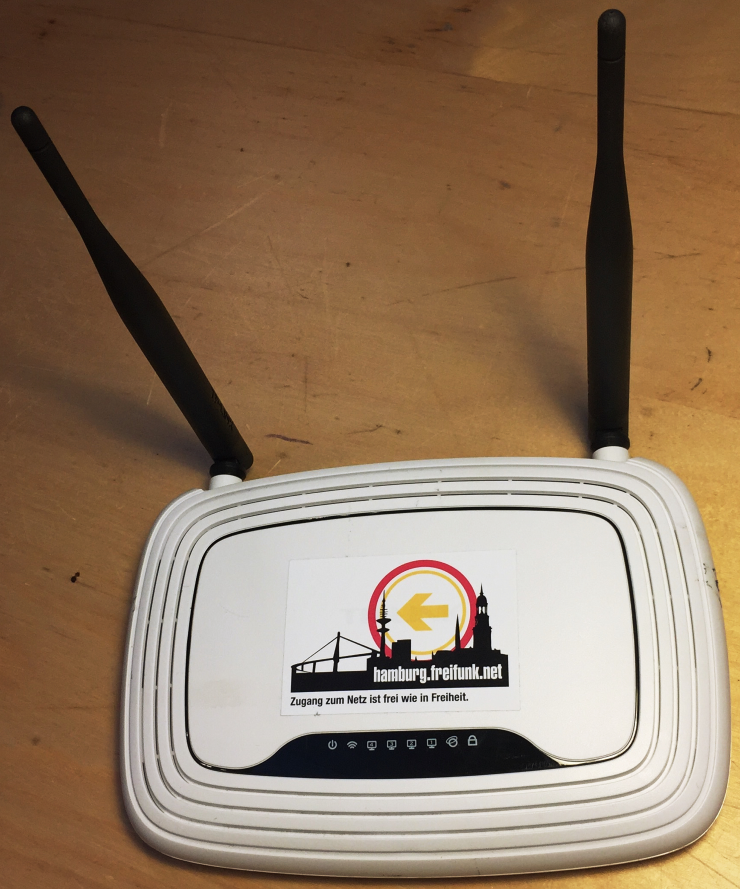
\includegraphics[width=\textwidth]{Bilder/841-cut}
        \end{center}
      \end{column}
      \begin{column}{0.4\textwidth}
        \begin{center}
          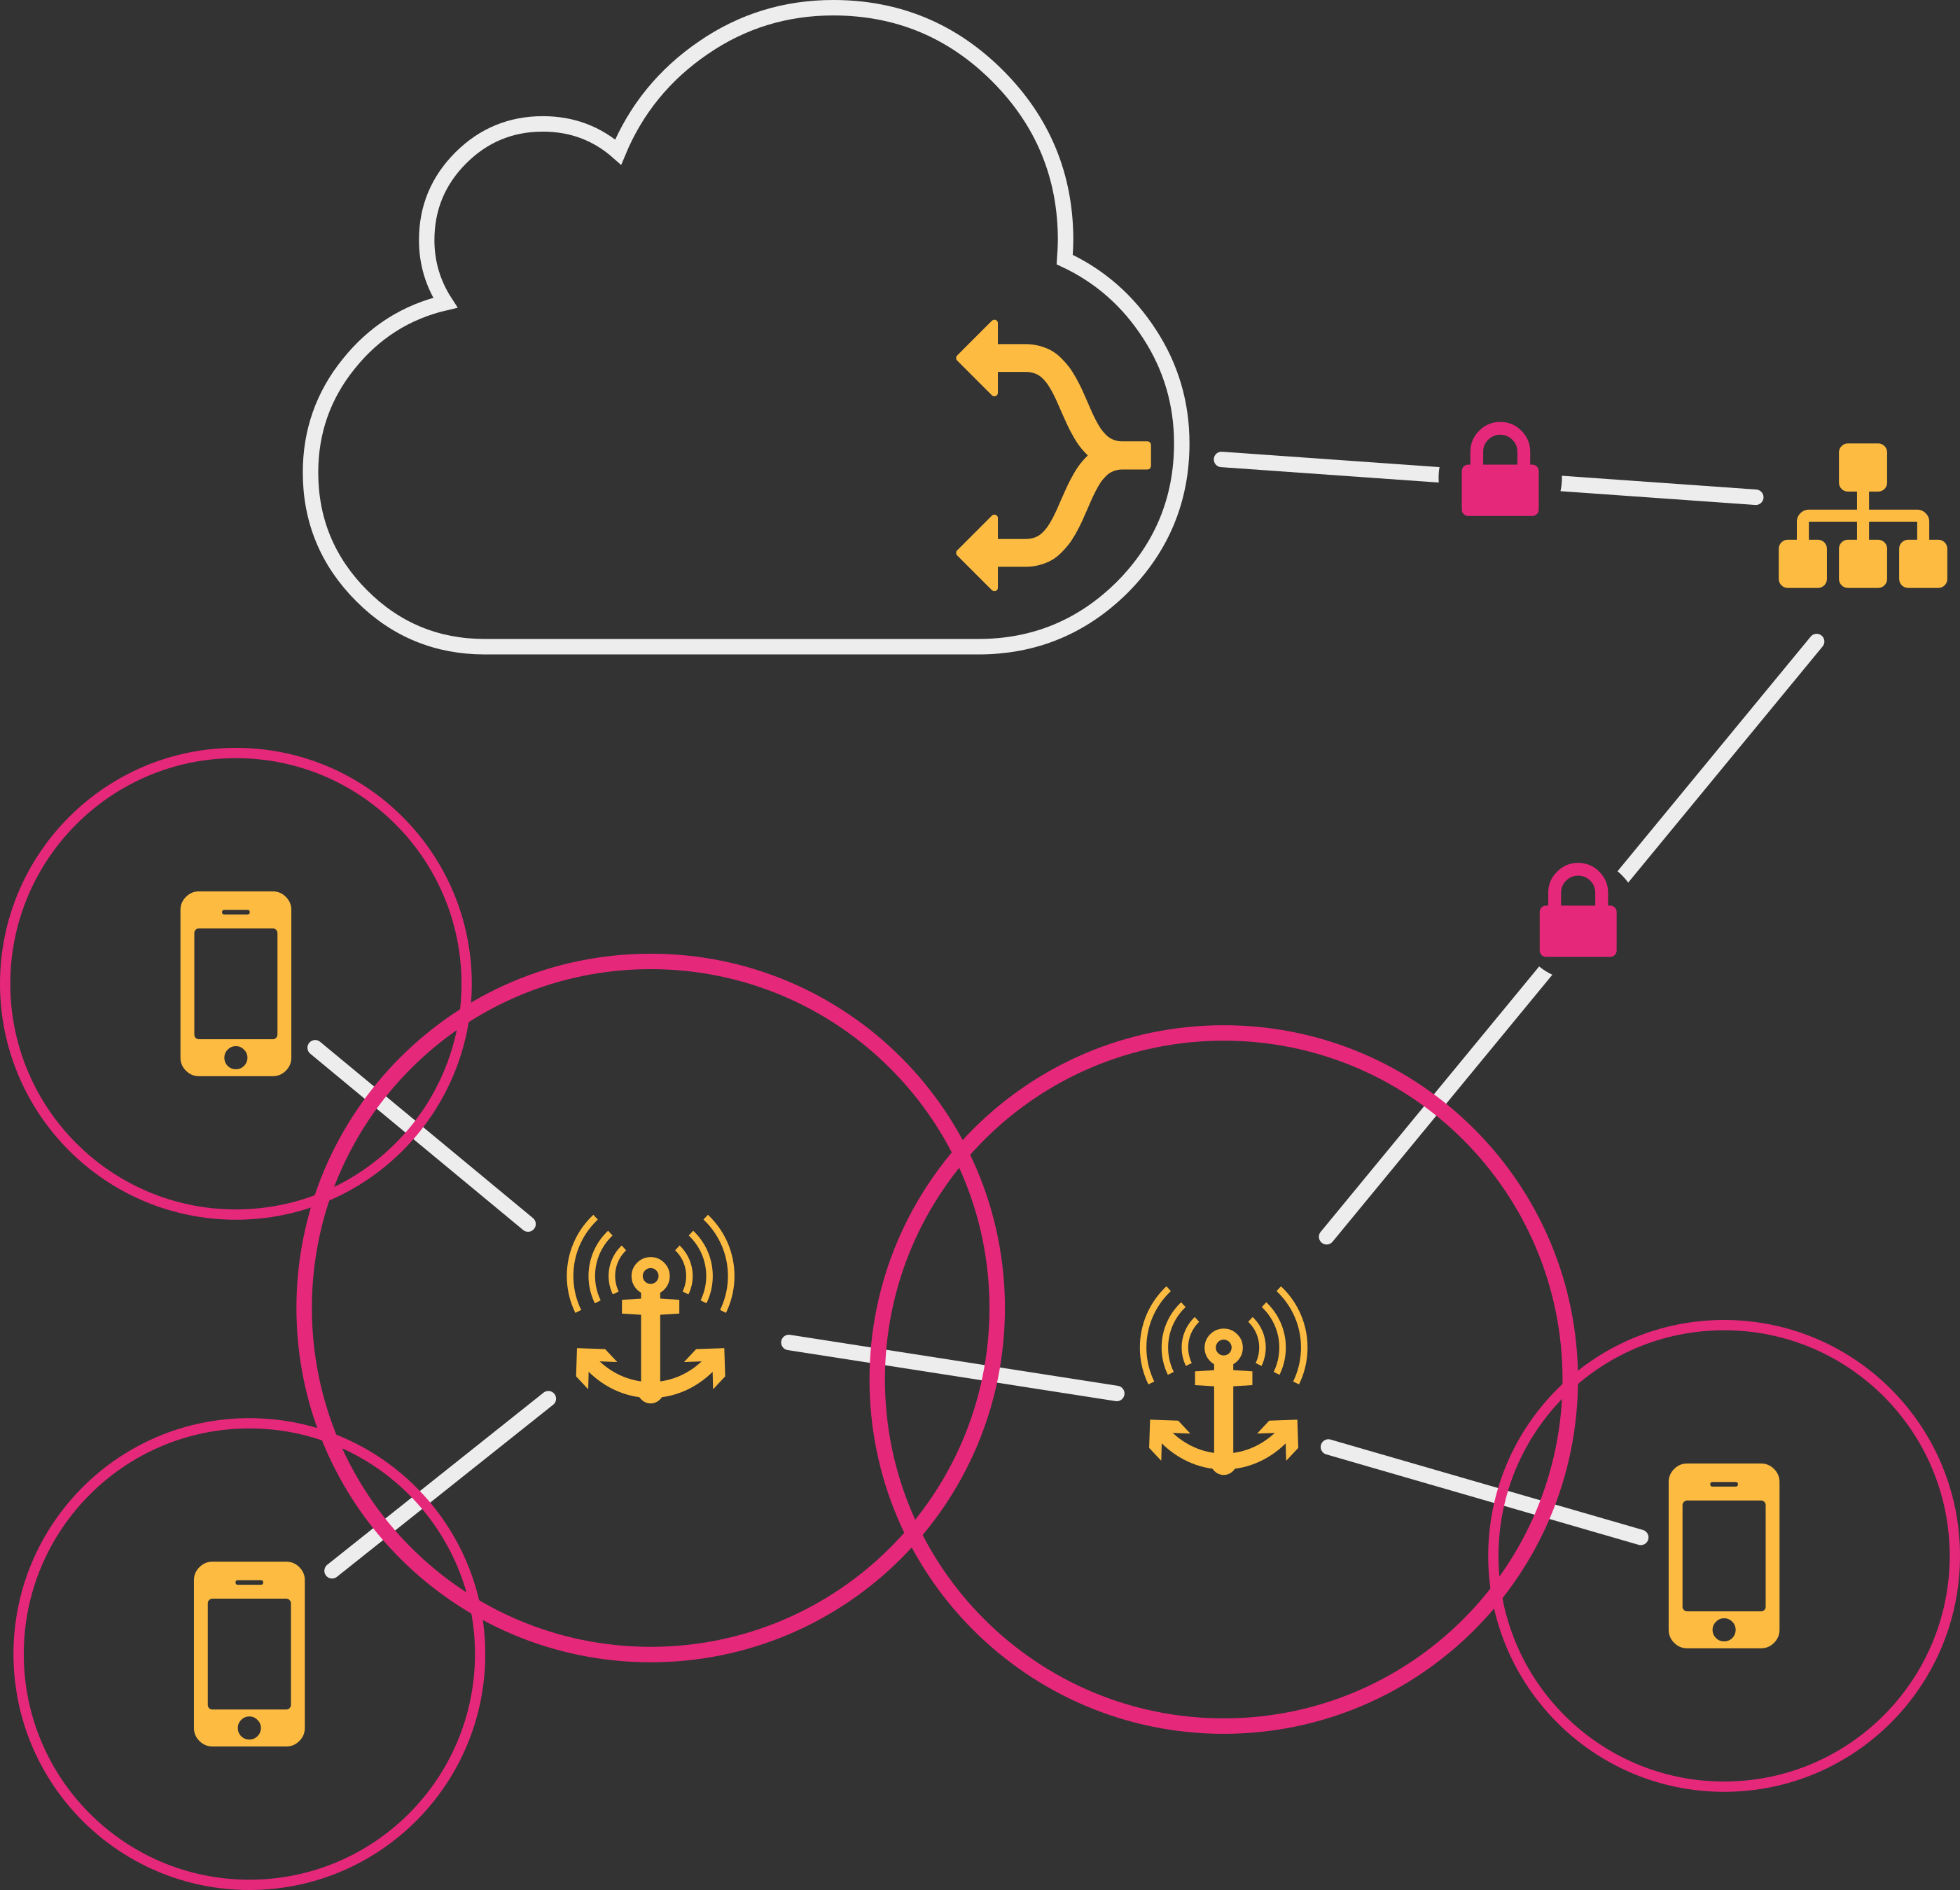
\includegraphics[width=\textwidth]{netz-klein}
        \end{center}
      \end{column}
    \end{columns}
  \end{frame}
  



  %-----------------
  \begin{frame}{\href{https://wiki.freifunk.net/Freifunk_Hamburg/Richtfunknetz}{Richtfunknetze}}
    \vspace{-1em}
    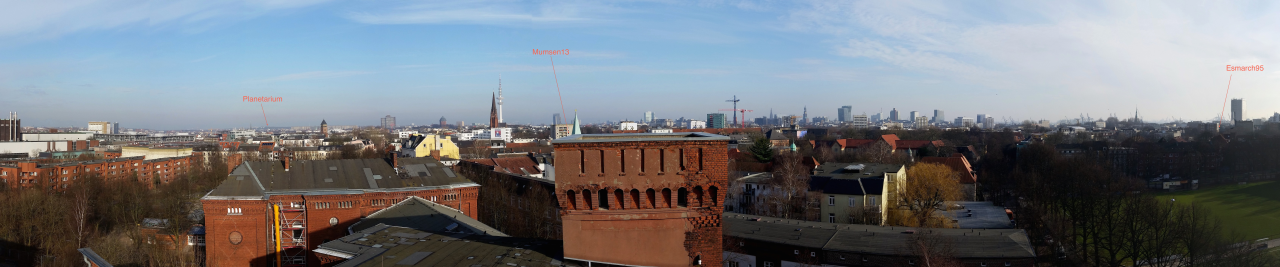
\includegraphics[width=\textwidth]{Bilder/fux}
    \begin{columns}
      \begin{column}{0.6\textwidth}
  \begin{itemize}
    \item Eigene Infrastruktur
    \begin{itemize}
      \item Unabhängigkeit von Internetprovidern
			\item Kostengünstiger als Kabelverlegung
    \end{itemize}
  \end{itemize}
      \end{column}
      \begin{column}{0.4\textwidth}
        \begin{center}
          \vspace{-3.5em}
          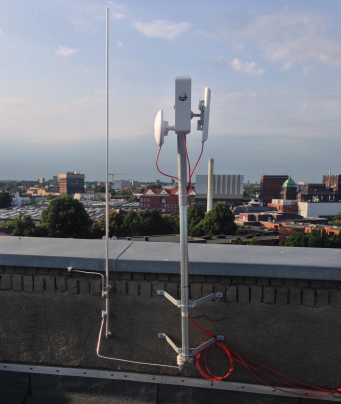
\includegraphics[width=.7\textwidth]{Bilder/richtfunkmast2}
        \end{center}
      \end{column}
    \end{columns}
  \end{frame}
	
	\begin{frame}{Freifunk Hamburg}
    \begin{itemize}
      \item Seit 2002 in Berlin, ca. 2003 zum ersten Mal in Hamburg
      \item 2012: Neustart. Wachstum auf mehr als 1100 Knoten und 2500 Nutzer*innen
      \item Früher: VPN ins Ausland
			\item Professionalisierung: Providerstatus, Autonomes System, Internetzugang in Deutschland 
			\item Keine laufenden Kosten, komplett aus Spenden finanziert
    \end{itemize}
  \end{frame}
	
	\begin{frame}{Freifunk für Geflüchtete}
    \begin{itemize}
      \item Ab 2013 in Hamburg: Versorgung vieler Flüchtlingsunterkünfte
      \item Deutschlandweites Thema für Freifunk
      \item Von technischer Spielerei zur Grundversorgung
			\item Konflikt: Wahrnehmung als Dienstleister \& bezahlte Ehrenamtliche \& langfriste Betreuung von Installationen
			\item "`\textit{Bitte realisieren Sie dringend eine WLAN-Versorung}"'
    \end{itemize}
    \begin{center}
          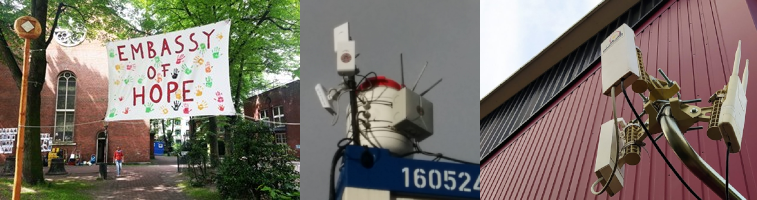
\includegraphics[width=0.7\textwidth]{Bilder/gefluechtete}
    \end{center}

  \end{frame}
	
	\begin{frame}{Organisationsform}
    \begin{itemize}
      \item Loser Zusammenschluss, unterstützt durch Vereine
      \item (Un)regelmäßige Plena mit Mehrheitsentscheid
			\item Aber auch: "`\textit{Wer macht, hat Recht}"'
      \item Steigende Komplexität führt zu größerer Einstiegshürde
      \item Vertrauensbasis: Wer hat/bekommt Zugriff worauf?
    \end{itemize}
  \end{frame}

\begin{frame}{Andere Initiativen}
    \begin{itemize}
      \item Im Rahmen der Professionalisierung entstanden:\\
            Freifunk Rheinland e.V. und andere lokale Vereine
      \item Italien: ninux.org als reines Intranet
      \item Spanien: guifi.net als offenes Netz mit kommerziellen Anbietern \& Kostenteilung
      \item USA: z.B. NYC Mesh mit Ehrenamtlichen \& Spendenempfehlung
    \end{itemize}
\end{frame}
  
  
    %-----------------
\begin{frame}{Politik}
    \vspace{-2em}
    \begin{columns}
      \begin{column}{0.6\textwidth}
        \begin{itemize}
          \item Förderung durch Städte und Kommunen
          \item Keine Gemeinnützigkeit
          \item Störerhaftung
          \item Freie Routerwahl
          \item Open Source \&\\
          \textit{Hackbare} Hardware
          \item Vorratsdatenspeicherung, Uploadfilter, Ende-zu-Ende-Verschlüsselung
   \end{itemize}
      \end{column}
      \begin{column}{0.4\textwidth}
        \begin{center}
          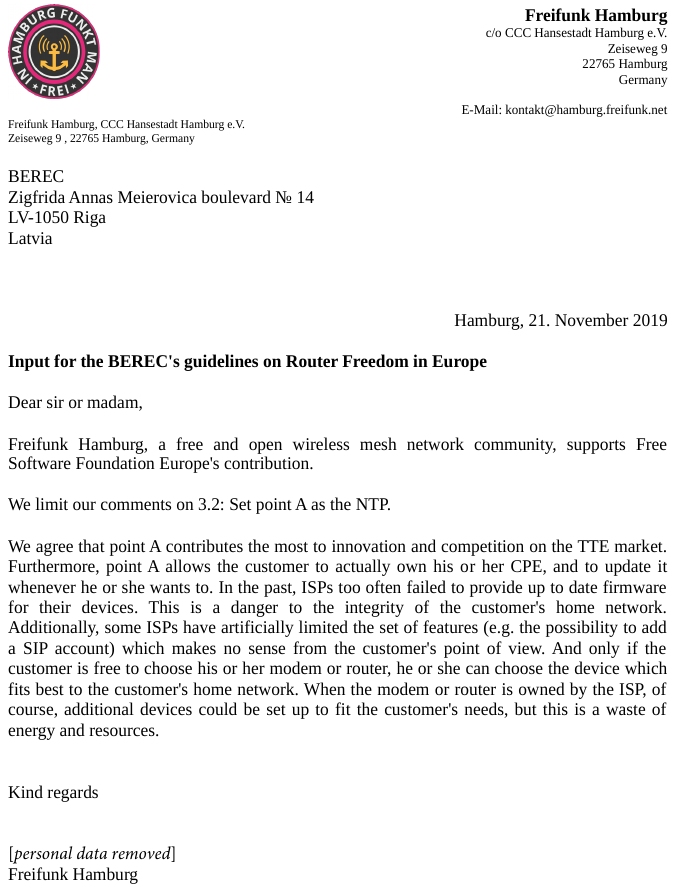
\includegraphics[height=0.8\textheight]{Bilder/berec}
        \end{center}
      \end{column}
    \end{columns}
  \end{frame}
  

  
  %-----------------
  \begin{frame}{WiFi4EU}
  \vspace{-1.5em}
  \begin{center}
    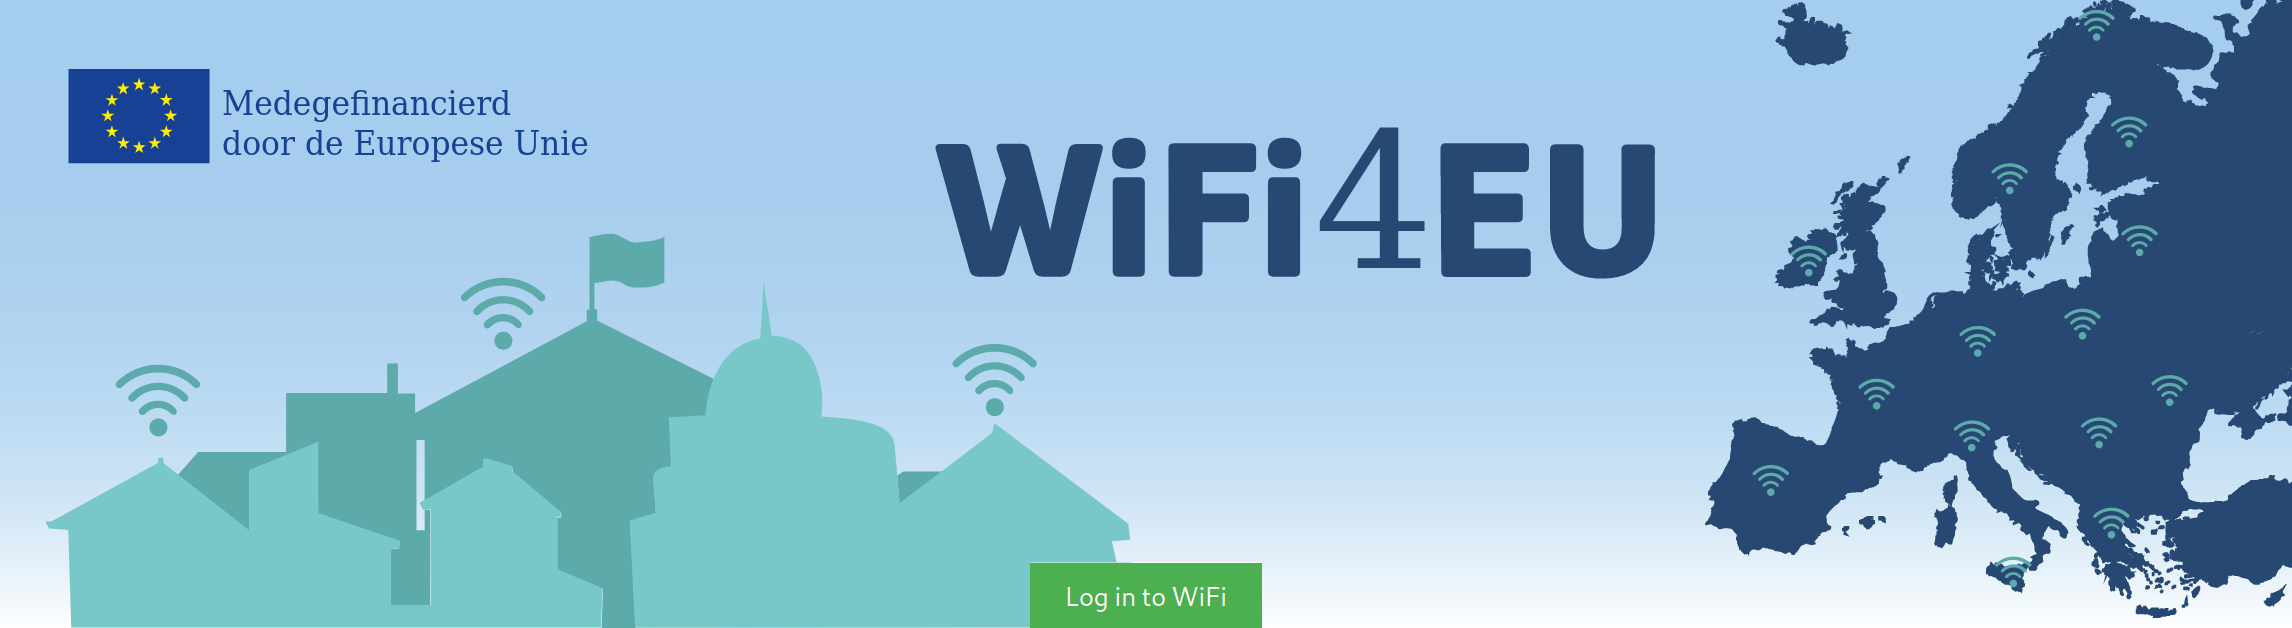
\includegraphics[width=0.8\textwidth]{Bilder/wifi4eu}
  \end{center}
  \begin{itemize}
   \item Förderprogramm der EU-Kommission:\\bis zu 15\,000 EUR, 8\,000 Gemeinden, drei Jahre
   \item Vorschaltseite inkl. Tracking-Codeschnipsel,\\
         überträgt eindeutige networkID \& Bildschirmauflösung
   \item Europaweites Authentifizierungssystem geplant
  \end{itemize}

% POST https://wifi4eucollectorprod.azurewebsites.net/api/PortalCollector HTTP/1.1
% User-Agent: Mozilla/5.0 (X11; Linux x86_64; rv:82.0) Gecko/20100101 Firefox/82.0
% Accept: application/json
% Accept-Language: de,en-US;q=0.7,en;q=0.3
% Content-type: application/json
% Content-Length: 680
% Origin: null
% Connection: keep-alive
% Host: wifi4eucollectorprod.azurewebsites.net
% 
% {"data":{"release":"2.0.3","metrics":{"DOMContentLoaded":828,"logoFinishedDownloading":901,"windowLoaded":1196},"visitor":{"viewport":{"width":2552,"height":1279},"image":{"branding":"banner","width":2536,"height":724.566650390625}},"validation":{"logo":{"srcCheck":true,"existsCheck":true,"typeCheck":true,"aspectRatioCheck":true,"widthToViewportCheck":true,"opacityCheck":true,"visibilityCheck":true,"overlapCheck":true,"completelyInViewPortAfterLoadingCheck":true},"installation":{"timer":true,"language":true}},"networkId":"123e4567-e89b-12d3-a456-426655440000","willExecuteNetworkMetricsTests":false},"networkMetricsData":{"networkId":"123e4567-e89b-12d3-a456-426655440000"}}

% {
%     "data": {
%         "release": "2.0.3",
%         "metrics": {
%             "DOMContentLoaded": 828,
%             "logoFinishedDownloading": 901,
%             "windowLoaded": 1196
%         },
%         "visitor": {
%             "viewport": {
%                 "width": 2552,
%                 "height": 1279
%             },
%             "image": {
%                 "branding": "banner",
%                 "width": 2536,
%                 "height": 724.566650390625
%             }
%         },
%         "validation": {
%             "logo": {
%                 "srcCheck": true,
%                 "existsCheck": true,
%                 "typeCheck": true,
%                 "aspectRatioCheck": true,
%                 "widthToViewportCheck": true,
%                 "opacityCheck": true,
%                 "visibilityCheck": true,
%                 "overlapCheck": true,
%                 "completelyInViewPortAfterLoadingCheck": true
%             },
%             "installation": {
%                 "timer": true,
%                 "language": true
%             }
%         },
%         "networkId": "123e4567-e89b-12d3-a456-426655440000",
%         "willExecuteNetworkMetricsTests": false
%     },
%     "networkMetricsData": {
%         "networkId": "123e4567-e89b-12d3-a456-426655440000"
%     }
% }
\end{frame}
  
\begin{frame}{Vorschaltseite (Captive Portal)}
\begin{itemize}
 \item Technisch nicht notwendig
 \item Verlängert die Anmeldeprozedur
 \item (Relativ) leicht zu umgehen
 \item Erst seit 2015 standardisiert, häufig kaputt
 \item Barriere für Geräte \& Apps
\end{itemize}
        \begin{center}
          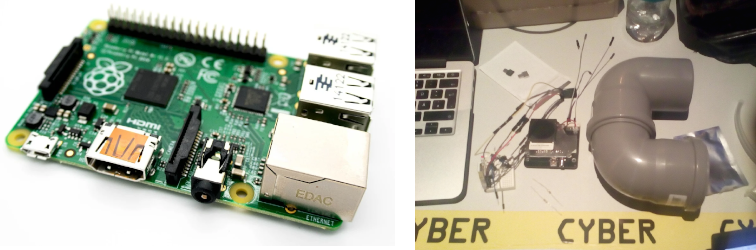
\includegraphics[width=0.8\textwidth]{Bilder/iot}
        \end{center}

\end{frame}
  
\begin{frame}{Vergleich verschiedener WLANs}
\begin{center}
\begin{tabular}{l|l|l|l}
WLAN & Vorschaltseite & Registrierungspflicht & Verschlüsselung\\\hline
Freifunk & nein & nein & nein\\
Wifi4EU & ja & geplant & nein\\
WIFIonICE & ja & nein & nein\\
div. Provider & ja & unterschiedlich & nein
\end{tabular}
\end{center}
\begin{itemize}
 \item Keine Verschlüsselung ist ein Problem.\\Wird besser mit \textit{Opportunistic Wireless Encryption}
 \item Keine gegenseitige Authentifizierung
 \item Clients sollten Ende-zu-Ende-verschlüsselt kommunizieren
\end{itemize}


\end{frame}
	
  
  %-----------------
  \begin{frame}{Vielen Dank!}
    \begin{columns}
      \begin{column}{0.5\textwidth}
        \centering
        \includesvg[width=3cm]{in-hamburg-funkt-man-frei}
      \end{column}
      \begin{column}{0.5\textwidth}
        \centering
        
\includegraphics[width=0.4\textwidth]{Bilder/qrcode-2020-11-12}
      \end{column}
    \end{columns}   
    \vspace{4em}
    \begin{itemize}
      \item \textbf{WWW} \href{https://hamburg.freifunk.net}{hamburg.freifunk.net}
      \item \textbf{E-Mail} \href{mailto:kontakt@hamburg.freifunk.net}{kontakt@hamburg.freifunk.net}
      %\item \textbf{Treffen} montags, 14-tägig\\\href{https://hamburg.freifunk.net/kalender}{\small https://hamburg.freifunk.net/kalender}
    \end{itemize}
  \end{frame}
  
  
\appendix
    %-----------------
  \begin{frame}[noframenumbering]{\tiny{www.}\huge{Knotenkarte}\tiny{.de}}
          \vspace{-1.5em}
    \begin{center}
      \includegraphics[width=\textwidth]{Bilder/knotenkarte-2020-11-12}
      \newline\tiny{Leaflet | \textrm{\textcopyright} CC-BY-SA OpenStreetMap, andere}
    \end{center}
    Mehr als 1100 Knoten in Hamburg, bis zu 2000 Geräte im Netz
  \end{frame}
  
\end{document}
